\chapter{Properties of Topological Spaces}

\section{Hausdorff Property}

\begin{definition}[First Separation Axiom, $T_1$]
A topological space \(X\) is said to satisfy the \emph{first separation axiom} (or to be a \emph{\(T_1\) space}) if for every pair of distinct points \(x,y \in X\), there exists an open set \(U \subseteq X\) such that
\[
x \in U \quad \text{and} \quad y \notin U.
\]
\end{definition}

\begin{proposition}
A topological space \(X\) satisfies the first separation axiom (\(T_1\)) if and only if every singleton set \(\{x\}\) is closed in \(X\).
\end{proposition}

\begin{proof}
\emph{(\(\Rightarrow\))} Assume \(X\) has the first separation property. Fix \(x \in X\). For each \(y \in X \smallsetminus \{x\}\), there exists an open set \(U_y\) with \(y \in U_y\) and \(x \notin U_y\). Then
\[
X \smallsetminus \{x\}
= \bigcup_{y \neq x} \{y\}
\subseteq \bigcup_{y \neq x} U_y
\subseteq X \smallsetminus \{x\}.
\]
Hence \(X \smallsetminus \{x\} = \bigcup_{y \neq x} U_y\) is open, so \(\{x\}\) is closed.

\emph{(\(\Leftarrow\))} Suppose every singleton is closed. Given \(x \neq y\), the set
\[
U := X \smallsetminus \{y\}
\]
is open, contains \(x\), and does not contain \(y\). Thus \(X\) has the first separation property.
\end{proof}

\begin{definition}[Hausdorff Space]
\label{def:Hausdorff}
A topological space \(X\) is called \emph{Hausdorff} (or said to satisfy the second separation axiom, \(T_2\)) if for every pair of distinct points \(x,y \in X\) there exist open neighborhoods \(U\) of \(x\) and \(V\) of \(y\) such that
\[
U \cap V = \varnothing.
\]
\end{definition}
\begin{example}
Every metrizable topological space is Hausdorff.  
Indeed, let \((X,d)\) be a metric space and take two distinct points \(x,y \in X\).  
Since \(d(x,y) = r > 0\), consider the open balls
\[
U := B_{r/2}(x), \qquad V := B_{r/2}(y).
\]
Then \(U\) and \(V\) are disjoint open neighborhoods of \(x\) and \(y\), respectively.  
Hence \((X,d)\) is Hausdorff.
\end{example}
Note that a topological space that is first separable may not necessarily be second separable:
\begin{example}
Consider \({\mathcal{T}}_{\text{ co-finite }}\), then \(X\) is first separable but not Hausdorff if \(X\) is infinite: Suppose on the contrary that for given \(x \neq  y\), there exists open sets \(U,V\) such that \(x \in  U,y \in  V\), and
\[
U \cap  V = \varnothing  \Rightarrow  X = X \smallsetminus  \left( {U \cap  V}\right)  = \left( {X \smallsetminus  U}\right)  \cup  \left( {X \smallsetminus  V}\right),
\]
implying that the union of two finite sets equals \(X\) which is infinite, so we have a contradiction.
\end{example}

We now explore some nice properties of a Hausdorff topological space:
\begin{proposition} If the topological space $(X, \mathcal{T})$ is Hausdorff, then all sequences \(\left\{  {x}_{n}\right\}\) in \(X\) has at most one limit.
\end{proposition}
\begin{proof} Suppose on the contrary that
\[
\left\{  {x}_{n}\right\}   \rightarrow  a,\;\left\{  {x}_{n}\right\}   \rightarrow  b\text{, with }a \neq  b
\]
By Hausdorff-ness, there exists \(U,V \in  \mathcal{T}\) and \(U \cap  V = \varnothing\) such that \(U \ni  a\) and \(V \ni  b\).

By tie openness of \(U\), there exists \(N\) such that \(\left\{  {{x}_{N},{x}_{N + 1},\ldots }\right\}   \subseteq  U\), since \(\left\{  {x}_{n}\right\}   \rightarrow  a \in  U\). Similarly, there exists \(M\) such that \(\left\{  {{x}_{M},{x}_{M + 1},\ldots }\right\}   \subseteq  V\). Let \(K = \max \{ M,N\}  + 1\), then \(\varnothing  \neq  U \cap  V \ni  {x}_{K}\), which is a contradiction.
\end{proof}

\begin{proposition} \label{prop:product_Hausdorff}
Let \(X\) and \(Y\) be Hausdorff spaces. Then the product space \(X \times Y\), equipped with the product topology, is Hausdorff.
\end{proposition}

\begin{proof}
Suppose \((x_{1},y_{1}) \neq (x_{2},y_{2})\) in \(X \times Y\). Then either \(x_{1} \neq x_{2}\) or \(y_{1} \neq y_{2}\).

Without loss of generality, assume \(x_{1} \neq x_{2}\). Since \(X\) is Hausdorff, there exist disjoint open sets \(U,V \subseteq X\) such that \(x_{1} \in U\) and \(x_{2} \in V\). Then
\[
(x_{1},y_{1}) \in U \times Y, 
\quad (x_{2},y_{2}) \in V \times Y,
\quad (U \times Y) \cap (V \times Y) = \varnothing.
\]

Thus \((x_{1},y_{1})\) and \((x_{2},y_{2})\) have disjoint open neighborhoods. Therefore, \(X \times Y\) is Hausdorff.
\end{proof}

The same argument applies if the second separation property is replaced by first separation property.

\begin{definition}[Topological embedding] \label{def:embedding}
A continuous injective map \(f : X \to Y\) between topological spaces is called a \emph{topological embedding} if 
\[
f : X \;\longrightarrow\; f(X)
\]
is a homeomorphism onto its image, where \(f(X)\) is equipped with the subspace topology from \(Y\).
\end{definition}

\begin{remark}
Equivalently, \(f\) is an embedding if it is continuous, injective, and for every open set \(U \subseteq X\), there exists an open set \(V \subseteq Y\) such that 
\[
U = f^{-1}(V) \cap X.
\]
\end{remark}

\begin{proposition} \label{prop:embedding_Hausdorff}
Let \(f : X \to Y\) be a topological embedding. If \(Y\) is Hausdorff, then \(X\) is Hausdorff.
\end{proposition}

\begin{proof}
Since \(f\) is an embedding, \(f : X \to f(X)\) is a homeomorphism onto its image, where \(f(X)\) is given the subspace topology from \(Y\).  

Take distinct points \(a,b \in X\). Then \(f(a) \neq f(b)\) in \(Y\). As \(Y\) is Hausdorff, there exist disjoint open sets \(U,V \subseteq Y\) with 
\[
f(a) \in U, \qquad f(b) \in V, \qquad U \cap V = \varnothing.
\]
It follows that \(U \cap f(X)\) and \(V \cap f(X)\) are disjoint open neighborhoods of \(f(a)\) and \(f(b)\) in \(f(X)\).  

By the homeomorphism \(f : X \to f(X)\), the preimages \(f^{-1}(U \cap f(X))\) and \(f^{-1}(V \cap f(X))\) are disjoint open neighborhoods of \(a\) and \(b\) in \(X\). Thus \(X\) is Hausdorff.
\end{proof}

\begin{remark}
If one only assumes that \(f\) is continuous and injective, the conclusion may fail.  
For example, let \(X\) be any non-Hausdorff space and let \(f : X \to \{*\}\) be the constant injective map into a one-point Hausdorff space. Then \(f\) is continuous and injective, but \(X\) is not Hausdorff. The embedding condition ensures that the topology of \(X\) is faithfully represented inside \(Y\).
\end{remark}

\begin{corollary} \label{cor:Hausdorff_invariant}
If \(f : X \to Y\) is a homeomorphism, then \(X\) is Hausdorff if and only if \(Y\) is Hausdorff.  
In particular, Hausdorff-ness is a \emph{topological property}, i.e., a property preserved under homeomorphism.
\end{corollary}

\section{Connectedness}

\begin{definition}[Connected space] \label{def:connected}
A topological space \((X, \mathcal{T})\) is said to be \emph{disconnected} if there exist non-empty open sets \(U,V \in \mathcal{T}\) such that
\[
U \cap V = \varnothing, \qquad U \cup V = X.
\]
If no such pair exists, then \(X\) is called \emph{connected}.
\end{definition}

\begin{proposition} \label{prop:connected_equiv}
For a topological space \((X, \mathcal{T})\), the following are equivalent:
\begin{enumerate}
    \item \(X\) is connected.
    \item The only subsets of \(X\) which are both open and closed are \(\varnothing\) and \(X\).
    \item Every continuous function \(f : X \to \{0,1\}\) (where \(\{0,1\}\) is equipped with the discrete topology) is constant.
\end{enumerate}
\end{proposition}

\begin{proof}
\noindent (1) $\Rightarrow$ (2):  
Suppose \(U \subseteq X\) is both open and closed. Then \(U\) and \(X \setminus U\) are disjoint open sets with 
\[
U \cup (X \setminus U) = X.
\]
By connectedness, either \(U = \varnothing\) or \(X \setminus U = \varnothing\). Hence \(U = \varnothing\) or \(U = X\).

\medskip

\noindent (2) $\Rightarrow$ (3):  
Let \(f : X \to \{0,1\}\) be continuous. Define
\[
U = f^{-1}(\{0\}), \qquad V = f^{-1}(\{1\}).
\]
Then \(U,V\) are open, disjoint, and \(U \cup V = X\). By (2), either \((U,V) = (X,\varnothing)\) or \((U,V) = (\varnothing,X)\). Thus \(f\) is constant.

\medskip

\noindent (3) $\Rightarrow$ (2):  
Suppose \(U \subseteq X\) is both open and closed. Define
\[
f(x) =
\begin{cases}
0, & x \in U, \\
1, & x \in X \setminus U.
\end{cases}
\]
This map \(f : X \to \{0,1\}\) is continuous. By (3), \(f\) is constant, hence \(U = \varnothing\) or \(U = X\).

\medskip

\noindent (2) $\Rightarrow$ (1):  
Suppose, for contradiction, that \(X\) is disconnected. Then there exist non-empty disjoint open sets \(U,V \subseteq X\) with \(U \cup V = X\). In this case, \(U = X \setminus V\) is both open and closed, contradicting (2). Hence \(X\) must be connected.
\end{proof}

\begin{corollary}
    The interval \(\left\lbrack  {a,b}\right\rbrack   \subseteq  \mathbb{R}\) is connnected
\end{corollary}

\begin{proof}
    Suppose on the contrary that there exists continuous function \(f : \left\lbrack  {a,b}\right\rbrack   \rightarrow  \{ 0,1\}\) that takes 2 values. Construct the mapping \(\widetilde{f} : \left\lbrack  {a,b}\right\rbrack   \rightarrow  \mathbb{R}\)

\[
\widetilde{f} : \left\lbrack  {a,b}\right\rbrack  \overset{f}{ \rightarrow  }\{ 0,1\} \overset{i}{ \rightarrow  }\mathbb{R}
\]

\[
\text{ with }\widetilde{f} = i \circ  f\text{. }
\]

Note that \(\{ 0,1\}  \subseteq  \mathbb{R}\) denotes the subspace topology, we imply the inclusion mapping \(i : \{ 0,1\}  \rightarrow  \mathbb{R}\) with \(s \mapsto  s\) is continuous. The composition of continuous mappings is continuous as well, i.e., \(\widetilde{f}\) is continuous.

Since the function \(f\) can take two values, there exists \(p,q \in  \left\lbrack  {a,b}\right\rbrack\) such that \(\widetilde{f}\left( p\right)  =\)  \(i \circ  f\left( p\right)  = 0\) and \(\widetilde{f}\left( q\right)  = i \circ  f\left( q\right)  = 1\). By intermediate value theorem, there exists \(r \in  \left\lbrack  {a,b}\right\rbrack\) such that \(\widetilde{f}\left( r\right)  = i \circ  f\left( r\right)  = 1/2\), which implies \(f\left( r\right)  = \frac{1}{2}\), which is a contradiction.
\end{proof} 

\begin{definition}[Connected subset] \label{def:connected_subset}
A non-empty subset \(S \subseteq X\) is connected if \((S, \mathcal{T}_S)\), where \(\mathcal{T}_S\) denotes the subspace topology on \(S\), is a connected topological space.

Equivalently, \(S \subseteq X\) is connected if, whenever \(U,V \subseteq X\) are open sets such that
\[
S \subseteq U \cup V, \qquad (U \cap V) \cap S = \varnothing,
\]
it follows that either \(U \cap S = \varnothing\) or \(V \cap S = \varnothing\).
\end{definition}

\begin{proposition} \label{prop:connected_image}
If \(f : X \to Y\) is continuous and \(A \subseteq X\) is connected, then \(f(A)\) is connected.  
In other words, the continuous image of a connected set is connected.
\end{proposition}

\begin{proof}
Suppose that \(U,V \subseteq Y\) are open sets such that
\[
f(A) \subseteq U \cup V, 
\qquad (U \cap V) \cap f(A) = \varnothing.
\]
Then
\[
A \subseteq f^{-1}(U) \cup f^{-1}(V), 
\qquad \bigl(f^{-1}(U) \cap A\bigr) \cap \bigl(f^{-1}(V) \cap A\bigr) = \varnothing.
\]

By the connectedness of \(A\), either \(f^{-1}(U) \cap A = \varnothing\) or \(f^{-1}(V) \cap A = \varnothing\).  
Therefore, either \(f(A) \cap U = \varnothing\) or \(f(A) \cap V = \varnothing\).  
Hence \(f(A)\) is connected.
\end{proof}

\begin{proposition} \label{prop:union_connected}
If \(\{A_i\}_{i \in I}\) is a family of connected subsets of \(X\) such that 
\[
A_i \cap A_j \neq \varnothing \quad \text{for all } i,j \in I,
\]
then the union \(\bigcup_{i \in I} A_i\) is connected.
\end{proposition}

\begin{proof}
Suppose the function \(f : \bigcup\limits_{i \in I} A_i \;\longrightarrow\; \{0,1\}\) is a continuous map. Then we imply that its restriction \({\left. f\right| }_{{A}_{i}} = f \circ  i : {A}_{i} \rightarrow  \{ 0,1\}\) is continuous for all \(i \in  I\). Thus \({\left. f\right| }_{{A}_{i}}\) is a constant for all \(i \in  I\). Due to the non-empty intersection of \({A}_{i},{A}_{j}\) for \(\forall i,j \in  I\), we imply \(f\) is constant. By \autoref{prop:connected_equiv},  \(\bigcup\limits_{i \in I} A_i\) is connected.
\end{proof}

\begin{exercise}
    Use \autoref{prop:connected_image} to give another proof. \emph{Hint.} Fix \(j \in I\). Construct a continuous map
\(
f_j : \bigcup_{i \in I} A_i \;\longrightarrow\; A_j.
\)
\end{exercise}


\begin{proposition} \label{prop:product_connected}
If \(X\) and \(Y\) are connected spaces, then the product space \(X \times Y\), equipped with the product topology, is connected.
\end{proposition}

\begin{proof}
Fix \(y_0 \in Y\). The subset
\[
B := X \times \{ y_0 \} \subseteq X \times Y
\]
is homeomorphic to \(X\), hence connected.  
Similarly, for each \(x \in X\), the subset
\[
C_x := \{x\} \times Y \subseteq X \times Y
\]
is homeomorphic to \(Y\), hence connected.  

Moreover, for each \(x \in X\),
\[
B \cap C_x = \{(x,y_0)\} \neq \varnothing.
\]
Thus, by \autoref{prop:union_connected}, the union
\[
B \cup \bigcup_{x \in X} C_x = X \times Y
\]
is connected.
\end{proof}

\begin{definition}[Path-Connectedness]\label{def:path_connectedness}
Let $(X, \mathcal{T})$ be a topological space.  

\begin{enumerate}
    \item A \emph{path} between two points \(x,y \in X\) is a continuous map 
    \[
        \tau : [0,1] \to X, \qquad \tau(0) = x,\; \tau(1) = y.
    \]
    
    \item The space \(X\) is said to be \emph{path-connected} if any two points in \(X\) can be joined by a path.
    
    \item A subset \(A \subseteq X\) is \emph{path-connected} if it is path-connected with respect to the subspace topology.  
    Equivalently, \(A\) is path-connected if for every pair of points \(x,y \in A\), there exists a continuous map 
    \[
        \tau : [0,1] \to A, \qquad \tau(0) = x,\; \tau(1) = y.
    \]
\end{enumerate}
\end{definition}

\begin{proposition}\label{prop:path_conn_implies_conn}
All path-connected spaces are connected.
\end{proposition}

\begin{proof}
Fix \(x \in X\). For each \(y \in X\), by path-connectedness there exists a continuous map 
\[
p_y : [0,1] \to X, \qquad p_y(0) = x, \; p_y(1) = y.
\]
Define
\[
C_y := p_y([0,1]) \subseteq X.
\]
By \autoref{prop:connected_image}, each \(C_y\) is connected, since it is the continuous image of the connected set \([0,1]\).  

Moreover, for any \(y,y' \in X\),
\[
C_y \cap C_{y'} \supseteq \{x\} \neq \varnothing.
\]
Thus the family \(\{C_y\}_{y \in X}\) is a collection of connected sets with non-empty mutual intersection. By \autoref{prop:union_connected}, we conclude that
\[
X = \bigcup_{y \in X} C_y
\]
is connected.
\end{proof}

\begin{exercise}
If \(A \subset B \subset \overline{A}\), then \(A\) connected implies \(B\) connected.  
(Hint: for every open \(U \subseteq X\), if \(U \cap A = \varnothing\), then also \(U \cap \overline{A} = \varnothing\).)
\end{exercise}

\begin{example}[Topologist's comb]
\label{ex:topologist_comb}
The converse of \autoref{prop:path_conn_implies_conn} is false.  
Consider the subset \(X \subseteq \mathbb{R}^2\) defined by
\[
X \;=\; 
\bigl( [0,1] \times \{0\} \bigr) 
\;\cup\; 
\bigcup_{n \in \mathbb{N}_{\geq 1}} \bigl( \{1/n\} \times [0,1] \bigr) 
\;\cup\; 
\{(0,1)\},
\]
where we take \(\mathbb{N}_{\geq 1} = \{1,2,3,\dots\}\).

This space, known as the \emph{Topologist's comb}, is connected but not path-connected
(see \autoref{fig:comb}).

\begin{figure}[h!]
\centering
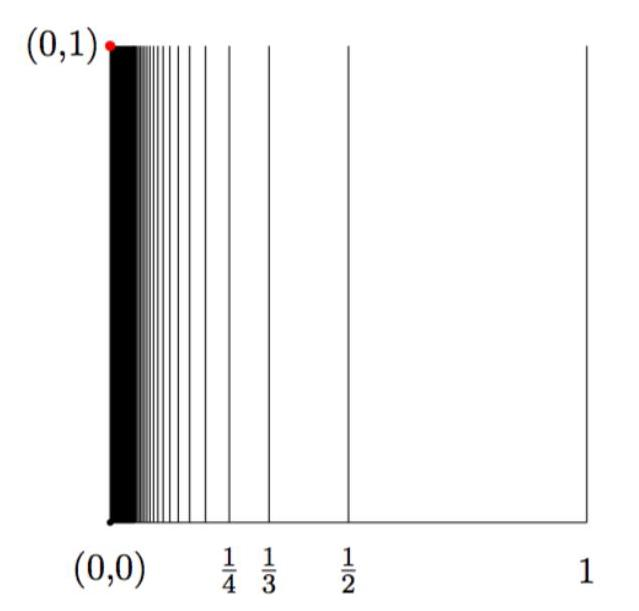
\includegraphics[width=0.5\textwidth]{images/Ch3_topologists_comb.jpg}
\caption{A connected but not path-connected space \(X\).}
\label{fig:comb}
\end{figure}

\begin{enumerate}
\item[\textbf{(a)}] 
\(X\) is not path-connected.  
Suppose there exists a path \(p : [0,1] \to X\) with
\[
p(0) = (0,1), \qquad p(1) = (x,y) \in X \setminus \{(0,1)\}.
\]
Define
\[
A := \{ t \in [0,1] \mid p(t) = (0,1) \}.
\]
We will show \(A = [0,1]\), i.e.\ the path must be constant.

\begin{enumerate}
\item[(i)] \(A\) is closed since it is the preimage of the closed singleton \(\{(0,1)\}\).  
\item[(ii)] \(A\) is open: fix \(t_0 \in A\). By continuity of \(p\), there exists \(\delta > 0\) such that
\[
\|p(t) - (0,1)\| < \tfrac{1}{2},
\qquad 
t \in [0,1] \cap (t_0 - \delta, t_0 + \delta).
\]
Thus \(p(t)\) cannot lie on the $x$-axis. Its $x$-coordinate must therefore belong to
\(\{0\} \cup \{1/n : n \geq 1\}\).  
Let \(I := [0,1] \cap (t_0 - \delta, t_0 + \delta)\). Consider the continuous function
\[
f := \pi_x \circ p : I \to \mathbb{R},
\]
where \(\pi_x(a,b) = a\) is the $x$-coordinate. Since \(I\) is connected, \(f(I)\) is connected.  
But \(f(I) \subseteq \{0\} \cup \{1/n : n \geq 1\}\), whose only connected subsets are singletons.  
Since \(f(t_0) = 0\), we deduce \(f(I) = \{0\}\). Hence \(p(t) = (0,1)\) for all \(t \in I\), i.e.\ \(I \subseteq A\).  
Thus \(A\) is open.
\end{enumerate}

Therefore \(A\) is nonempty, closed, and open in the connected interval \([0,1]\), so \(A = [0,1]\).  
Hence any such path is constant, and no path connects \((0,1)\) to another point of \(X\).

\item[\textbf{(b)}] 
Nonetheless, \(X\) is connected. (Proof omitted here, but it relies on showing that any separation would disconnect the horizontal interval from the vertical combs, which is impossible.)
\end{enumerate}
\end{example}

\section{Compactness}

Compactness generalizes the Euclidean notion of “closed and bounded” subsets of \(\mathbb{R}^n\).

\begin{definition}[Compactness]
\label{def:compactness}
Let \((X, \mathcal{T})\) be a topological space.  

\begin{enumerate}
\item 
A collection \(\mathcal{U} = \{U_i \mid i \in I\}\) of open sets is called an \emph{open cover} of \(X\) if
\[
X \;=\; \bigcup_{i \in I} U_i.
\]

\item 
A \emph{subcover} of \(\mathcal{U}\) is a subfamily
\[
\mathcal{U}' = \{ U_j \mid j \in J \}, \qquad J \subseteq I,
\]
such that
\[
X \;=\; \bigcup_{j \in J} U_j.
\]

\item 
If \(J\) is finite, then \(\mathcal{U}'\) is called a \emph{finite subcover}.
\end{enumerate}

We say that \(X\) is \emph{compact} if every open cover of \(X\) admits a finite subcover i.e. \(X \;=\; \bigcup\limits_{j = 1}^n U_j.\)

\medskip
If \(A \subseteq X\) is equipped with the subspace topology, then \(A\) is compact if and only if,
for every collection of open sets \(\{U_i\}_{i \in I}\) in \(X\) such that
\[
A \;\subseteq\; \bigcup_{i \in I} U_i,
\]
there exists a finite subcollection
\[
A \;\subseteq\; \bigcup_{k=1}^n U_{i_k}.
\]
\end{definition}

\begin{proposition}[Finite Intersection Property]
\label{prop:FIP}
Let \(X\) be a topological space. The following are equivalent:
\begin{enumerate}
\item \(X\) is compact.
\item If \(\{V_i \mid i \in I\}\) is a collection of closed subsets of \(X\) with the property that
\[
\bigcap_{j \in J} V_j \;\neq\; \varnothing, 
\qquad \text{for all finite } J \subseteq I,
\]
then
\[
\bigcap_{i \in I} V_i \;\neq\; \varnothing.
\]
\end{enumerate}
\end{proposition}

Compactness is an \emph{intrinsic} property of a space: it depends only on the topology of \(X\), not on how \(X\) may be embedded into some larger space.

\begin{example}
\leavevmode
\begin{enumerate}
\item[\textbf{1.}] 
If \(X \subseteq \mathbb{R}^n\), then \(X\) is compact if and only if \(X\) is closed and bounded.  
(This is the classical \href{https://en.wikipedia.org/wiki/Heine%E2%80%93Borel_theorem}{\emph{Heine--Borel theorem}}.)

\item[\textbf{2.}] 
Let \(K \subseteq \mathbb{R}^n\) be compact, and define
\[
\mathcal{C}(K) \;=\; \{\, f : K \to \mathbb{R} \;\mid\; f \text{ continuous} \,\}.
\]
Equip \(\mathcal{C}(K)\) with the \(\infty\)-norm
\[
\|f\|_\infty \;=\; \sup_{k \in K} |f(k)|.
\]
This induces the metric space \(\bigl(\mathcal{C}(K), d_\infty \bigr)\), where
\[
d_\infty(f,g) \;=\; \|f-g\|_\infty,
\]
which is in fact a \href{https://en.wikipedia.org/wiki/Banach_space}{Banach space} (a complete normed vector space).

A subset \(\mathcal{J} \subseteq \mathcal{C}(K)\) is compact if and only if it is
\[
\bigl[\text{closed, bounded, and equicontinuous}\bigr]
\]
(where \emph{equicontinuous} means: for every \(\varepsilon > 0\), there exists \(\delta > 0\) such that 
\(|f(x)-f(y)| < \varepsilon\) for all \(f \in \mathcal{J}\) whenever \(\|x-y\| < \delta\)).  
(This is the celebrated \href{https://en.wikipedia.org/wiki/Arzel%C3%A0%E2%80%93Ascoli_theorem}{\emph{Arzelà--Ascoli theorem}}.)

\medskip
This shows that in infinite-dimensional spaces, compactness is no longer the same as closedness plus boundedness.
\end{enumerate}
\end{example}

\begin{proposition}
\label{prop:closed_subsets_compact}
Let \(X\) be a compact space. Then every closed subset \(A \subseteq X\) is compact.
\end{proposition}

\begin{proof}
Let \(\{V_i \mid i \in I\}\) be a collection of closed subsets of \(A\) such that 
\[
\bigcap_{j \in J} V_j \;\neq\; \varnothing 
\quad\text{for all finite } J \subseteq I.
\]
Since \(A\) is closed in \(X\), each \(V_i\) can be written as \(V_i = A \cap W_i\) for some closed set \(W_i \subseteq X\).  
Thus the family \(\{W_i \mid i \in I\}\) has the \hyperref[prop:FIP]{finite intersection property} in \(X\).  

By compactness of \(X\), we deduce
\[
\bigcap_{i \in I} W_i \;\neq\; \varnothing.
\]
Intersecting with \(A\), we get
\[
\bigcap_{i \in I} V_i 
= A \cap \bigcap_{i \in I} W_i 
\;\neq\; \varnothing.
\]

Hence \(A\) is compact by the \hyperref[prop:FIP]{finite intersection property}.
\end{proof}

Now consider the reverse direction of \autoref{prop:closed_subsets_compact}, i.e., are all compact subsets \(K \subseteq  X\) closed in \(X\) ?

In general, the converse does not hold. Note that \(K = \{ x\}\) is compact for any topology \(X\). However, there are some topologies such that a singleton is not closed.

In order to obtain the converse of \autoref{prop:closed_subsets_compact}, we impose \hyperlink{def:Hausdorff}{the second separation axiom}.

\begin{proposition}[Point--compact set separation in Hausdorff spaces]
\label{prop:point_compact_separation}
Let \(X\) be Hausdorff, let \(K\subseteq X\) be compact, and let \(x\in X\setminus K\).
Then there exist open sets \(U,V\subseteq X\) such that
\[
K\subseteq U,\qquad x\in V,\qquad U\cap V=\varnothing.
\]
\end{proposition}

\begin{proof}
Let \(k \in K\). Since \(X\) is Hausdorff, there exist open sets \(U_k \ni k\) and \(V_k \ni x\) with
\(U_k \cap V_k = \varnothing\).
Then \(\{U_k\}_{k \in K}\) is an open cover of \(K\).
By compactness of \(K\), there exist \(k_1,\dots,k_n \in K\) such that
\(K \subseteq \bigcup_{i=1}^n U_{k_i}\).
Define
\[
U := \bigcup_{i=1}^n U_{k_i}
\qquad\text{and}\qquad
V := \bigcap_{i=1}^n V_{k_i}.
\]
Both \(U\) and \(V\) are open; clearly \(K \subseteq U\) and \(x \in V\).
Moreover,
\[
U \cap V \;\subseteq\; \bigcup_{i=1}^n \bigl(U_{k_i} \cap V_{k_i}\bigr) \;=\; \varnothing,
\]
so \(U\) and \(V\) are disjoint.
This proves the claim.
\end{proof}

By making use of this separation axiom, we obtain the converse of \autoref{prop:closed_subsets_compact}:

\begin{corollary}\label{cor:compact_closed_in_Hausdorff}
If \(X\) is Hausdorff and \(K \subseteq X\) is compact, then \(K\) is closed in \(X\).
\end{corollary}

\begin{proof}
Fix \(x \in X \setminus K\).
By \autoref{prop:point_compact_separation}, there exist open sets \(U,V \subseteq X\) such that
\(K \subseteq U\), \(x \in V\), and \(U \cap V = \varnothing\).
Hence \(V \subseteq X \setminus U \subseteq X \setminus K\),
so \(x\) has an open neighborhood contained in \(X \setminus K\).
Since this holds for every \(x \in X \setminus K\), the complement \(X \setminus K\) is open, and thus \(K\) is closed.
\end{proof}

\subsection{Continuous Functions on Compact Space}

\begin{proposition}\label{prop:image_of_compact_is_compact}
Let \(f : X \to Y\) be a continuous map between topological spaces, and let \(A \subseteq X\) be compact.  
Then \(f(A) \subseteq Y\) is compact.
\end{proposition}

\begin{proof}
Let \(\{U_i \mid i \in I\}\) be an open cover of \(f(A)\), i.e.
\[
f(A) \;\subseteq\; \bigcup_{i \in I} U_i, 
\qquad U_i \in \mathcal{T}_Y.
\]
Then the preimages \(\{ f^{-1}(U_i) \mid i \in I \}\) form an open cover of \(A\), since
\[
A \;\subseteq\; f^{-1}\!\Bigl(\,\bigcup_{i \in I} U_i \Bigr) 
= \bigcup_{i \in I} f^{-1}(U_i).
\]
By compactness of \(A\), there exists a finite subcover
\[
A \;\subseteq\; \bigcup_{k=1}^n f^{-1}(U_{i_k}).
\]
Applying \(f\) gives
\[
f(A) \;\subseteq\; f\!\Bigl( \,\bigcup_{k=1}^n f^{-1}(U_{i_k}) \Bigr) 
\;\subseteq\; \bigcup_{k=1}^n U_{i_k}.
\]
Thus \(f(A)\) has a finite subcover, and hence is compact.
\end{proof}

\begin{corollary}\label{cor:extreme_value}
\begin{enumerate}
\item[\textbf{1.}]
Suppose \(X\) is compact, and \(f : X \to \mathbb{R}\) is continuous.  
Then \(f(X)\) is closed and bounded.  
In particular, there exist \(m, M \in X\) such that
\[
f(m) \;\leq\; f(x) \;\leq\; f(M), \qquad \forall x \in X.
\]

\item[\textbf{2.}]
Suppose moreover that \(X\) is connected.  
Then
\[
f(X) \;=\; [\, f(m), \, f(M) \,].
\]
\end{enumerate}
\end{corollary}

\begin{proof}
(1) By \autoref{prop:image_of_compact_is_compact}, \(f(X)\) is compact in \(\mathbb{R}\).  
By the Heine--Borel theorem, compact subsets of \(\mathbb{R}\) are closed and bounded.  
Hence \(f(X)\) attains both its minimum and maximum values at some points \(m, M \in X\).  

\smallskip
(2) If \(X\) is also connected, then by continuity of \(f\), the image \(f(X)\) is connected.  
But the only connected subsets of \(\mathbb{R}\) are intervals.  
Since \(f(X)\) is compact, it must be a closed interval.  
Thus
\[
f(X) = [\, f(m), f(M) \,]. \qedhere
\]
\end{proof}

\begin{lemma}[Tube Lemma]\label{lem:tube}
Let \(X, Y\) be topological spaces, and assume \(Y\) is compact.  
If \(W \subseteq X \times Y\) is open and 
\[
\{x_0\} \times Y \subseteq W,
\]
then there exists an open neighborhood \(U \subseteq X\) of \(x_0\) such that 
\[
U \times Y \subseteq W.
\]
\end{lemma}

\begin{proof}
For each \(y \in Y\), since \((x_0, y) \in W\) and \(W\) is open, there exist neighborhoods 
\(U_y \subseteq X\), \(V_y \subseteq Y\) such that
\[
(x_0, y) \in U_y \times V_y \subseteq W.
\]
Then \(\{V_y : y \in Y\}\) is an open cover of \(Y\).  
By compactness, there exist finitely many points \(y_1, \ldots, y_n \in Y\) such that
\[
Y \subseteq V_{y_1} \cup \cdots \cup V_{y_n}.
\]
Define
\[
U \;:=\; U_{y_1} \cap \cdots \cap U_{y_n}.
\]
Then \(U\) is an open neighborhood of \(x_0\), and we have
\[
U \times Y \subseteq (U_{y_1} \times V_{y_1}) \cup \cdots \cup (U_{y_n} \times V_{y_n})
\subseteq W.
\]
Thus the claim follows.
\end{proof}

\begin{theorem}[Tychonoff for finite products]\label{thm:product_compact}
Let \(X,Y\) be topological spaces. Then \(X \times Y\) is compact under the product topology 
if and only if both \(X\) and \(Y\) are compact.
\end{theorem}

\begin{proof}
\noindent(\(\Rightarrow\)) Suppose \(X \times Y\) is compact.  
Consider the projection maps
\[
p_X : X \times Y \to X, 
\qquad 
p_Y : X \times Y \to Y.
\]
These are continuous, so by \autoref{prop:image_of_compact_is_compact} the images
\(p_X(X \times Y) = X\) and \(p_Y(X \times Y) = Y\) are compact.

\smallskip
\noindent(\(\Leftarrow\)) Suppose \(X\) and \(Y\) are compact.  
Let \(\{W_i\}_{i \in I}\) be an open cover of \(X \times Y\).  
Fix \(x_0 \in X\). Then \(\{x_0\} \times Y\) is compact, so it is covered by finitely many 
\(W_{i_1}, \dots, W_{i_n}\).  
Define
\[
W := W_{i_1} \cup \cdots \cup W_{i_n},
\]
which is an open neighborhood of \(\{x_0\} \times Y\).  
By the \hyperref[lem:tube]{tube lemma}, there exists an open neighborhood \(U_{x_0} \subseteq X\) of \(x_0\) such that
\[
U_{x_0} \times Y \subseteq W.
\]

Thus \(\{U_{x_0} : x_0 \in X\}\) is an open cover of \(X\).  
By compactness of \(X\), choose finitely many \(x_1,\dots,x_m \in X\) such that
\[
X = U_{x_1} \cup \cdots \cup U_{x_m}.
\]
It follows that
\[
X \times Y \subseteq \bigcup_{\ell=1}^m \bigl(U_{x_\ell} \times Y \bigr) 
\subseteq \bigcup_{\ell=1}^m \bigl(W_{i_1} \cup \cdots \cup W_{i_n}\bigr),
\]
a finite union of members of the original cover.  
Therefore \(X \times Y\) is compact.
\end{proof}

\begin{theorem}\label{thm:compact_hausdorff_homeo}
Suppose that \(X\) is compact, \(Y\) is Hausdorff, and 
\(f : X \to Y\) is a continuous bijection. Then \(f\) is a homeomorphism.
\end{theorem}

\begin{proof}
Since \(f\) is bijective, to show that \(f^{-1}\) is continuous it suffices to prove that
\((f^{-1})^{-1}(V) = f(V)\) is closed in \(Y\) for every closed set \(V \subseteq X\).


Let \(V \subseteq X\) be closed. Then \(V\) is compact since closed subsets of a compact space are compact, by \autoref{prop:closed_subsets_compact}.  
By continuity of \(f\) and \autoref{prop:image_of_compact_is_compact}.  , the image \(f(V)\) is compact in \(Y\).
Since \(Y\) is Hausdorff, compact subsets are closed (see \autoref{cor:compact_closed_in_Hausdorff}).  
Hence \(f(V)\) is closed in \(Y\).

Thus, for every closed set \(V \subseteq X\), the image \(f(V)\) is closed in \(Y\).  
This is exactly the statement that \(f^{-1}\) is continuous. Therefore \(f\) is a homeomorphism.
\end{proof}

\begin{corollary}\label{cor:injective_compact_homeo_onto_image}
If \(X\) is compact, \(Y\) is Hausdorff, and \(f : X \to Y\) is injective and continuous, then
\[
f : X \longrightarrow f(X)
\]
is a homeomorphism (where \(f(X)\) carries the subspace topology from \(Y\)).
\end{corollary}

\begin{example}[Second proof of \(S^{1}\times S^{1}\) is isomorphic to a torus]\label{ex:S1xS1_torus}
Identify \(S^{1}=\{e^{i\theta} : \theta\in[0,2\pi)\}\subset\mathbb{C}\).
Define
\[
f : S^{1}\times S^{1} \longrightarrow \mathbb{R}^{3},\qquad
\bigl(e^{i\theta},e^{i\phi}\bigr) \longmapsto
\bigl((R+r\cos\theta)\cos\phi,\ (R+r\cos\theta)\sin\phi,\ r\sin\theta\bigr),
\]
with parameters \(R>r>0\). Let \(T:=f(S^{1}\times S^{1})\subset\mathbb{R}^{3}\).

\begin{itemize}
\item \(X:=S^{1}\times S^{1}\) is compact, and \(\mathbb{R}^{3}\) is Hausdorff.
\item \(f\) is continuous and injective (this is the standard parametrization of a ring torus).
\item The image \(T\) is the (embedded) \emph{ring torus} in \(\mathbb{R}^{3}\) with major radius \(R\) and minor radius \(r\).
\end{itemize}

By \autoref{cor:injective_compact_homeo_onto_image}, a continuous injective map from a compact space into a Hausdorff space
is a homeomorphism onto its image. Hence \(f: S^{1}\times S^{1}\to T\) is a homeomorphism, i.e.
\[
S^{1}\times S^{1}\ \cong\ T\ \subset \mathbb{R}^{3}.
\]
\end{example}



\begin{definition}[Sequential Compactness]\label{def:sequential_compact}
A topological space \(X\) is \emph{sequentially compact} if every sequence in \(X\) admits a convergent subsequence, i.e., for every sequence \(\{x_n\}_{n \in \mathbb{N}} \subseteq X\), there exists a subsequence \(\{x_{n_k}\}_{k \in \mathbb{N}}\) and a point \(x \in X\) such that 
\[
x_{n_k} \to x \quad \text{in } X.
\]
\end{definition}

In a metric space \((X,d)\), compactness and sequential compactness are equivalent.  
In particular, for \(\mathbb{R}^n\) with the Euclidean metric, a subset is compact 
if and only if it is sequentially compact. (Check notes for MAT3006)

\begin{remark}
For general topological spaces, compactness and sequential compactness need not coincide.  
For example, the first uncountable ordinal \(\omega_1\) with the order topology is compact but not sequentially compact.
\end{remark}